\documentclass{article}

\usepackage{graphicx}
\usepackage[T1]{fontenc}


\title{Lab 7}
\author{Filip Jędrzejewski}

\begin{document}
	\maketitle
	
	\section*{Zadanie 1}
	
	\subsection*{Opis problemu}

	Celem zadania było obliczenie całki:

	\begin{equation}
		\int_{0}^{1} \frac{4}{1 + x^2} \,dx
	\end{equation}

	korzystając z kwadratur adaptacyjnych trapezów oraz kwadratur adaptacyjnych Gaussa-Kronroda.


	\subsection*{Całkowanie numeryczne}

	W celu zastosowania kwadratur adaptacyjnych trapezów użyto następującej funkcji:

	\begin{verbatim}
		import scipy.integrate as scint
		def trapzAdaptive(f, a, b, eps):
    result = scint.quad_vec(f, a, b, epsrel=eps, quadrature='trapezoid', full_output=True)
    toReturn = (result[0], result[2].neval)
    return toReturn
	\end{verbatim}
	
	Natomiast dla kwadratur adaptacyjnych Gaussa-Kronroda użyto:

	\begin{verbatim}
		def gaussKronrodAdaptive(f, a, b, eps):
    result = scint.quad_vec(f, a, b, epsrel=eps, quadrature='gk21', full_output=True)
    toReturn = (result[0], result[2].neval)
    return toReturn
	\end{verbatim}

	Obie funkcje przyjmują funkcję, która będzie całkowana, granice przedziału całkowania $[a,b]$ oraz \texttt{eps}, czyli dopuszczalny błąd (tolerancję).

	Funkcje zwracają krotkę zawierającą wynik całki oraz liczbę ewaluacji funkcji podcałkowej.

	
	\subsection*{Wykresy}

	Dla każdej metody stworzono wykres wartości bezwzględnej błędu względnego w zależności od liczby ewaluacji funkcji podcałkowej. Na tę liczbę wpływano poprzez zmienianie parametru \texttt{eps} w funkcji liczącej całkę w zakresie od $10^{0}$ do $10^{-14}$. Wyniki dodano do wykresu z poprzedniego laboratorium (6):

	\begin{figure}[h]
		\centering
		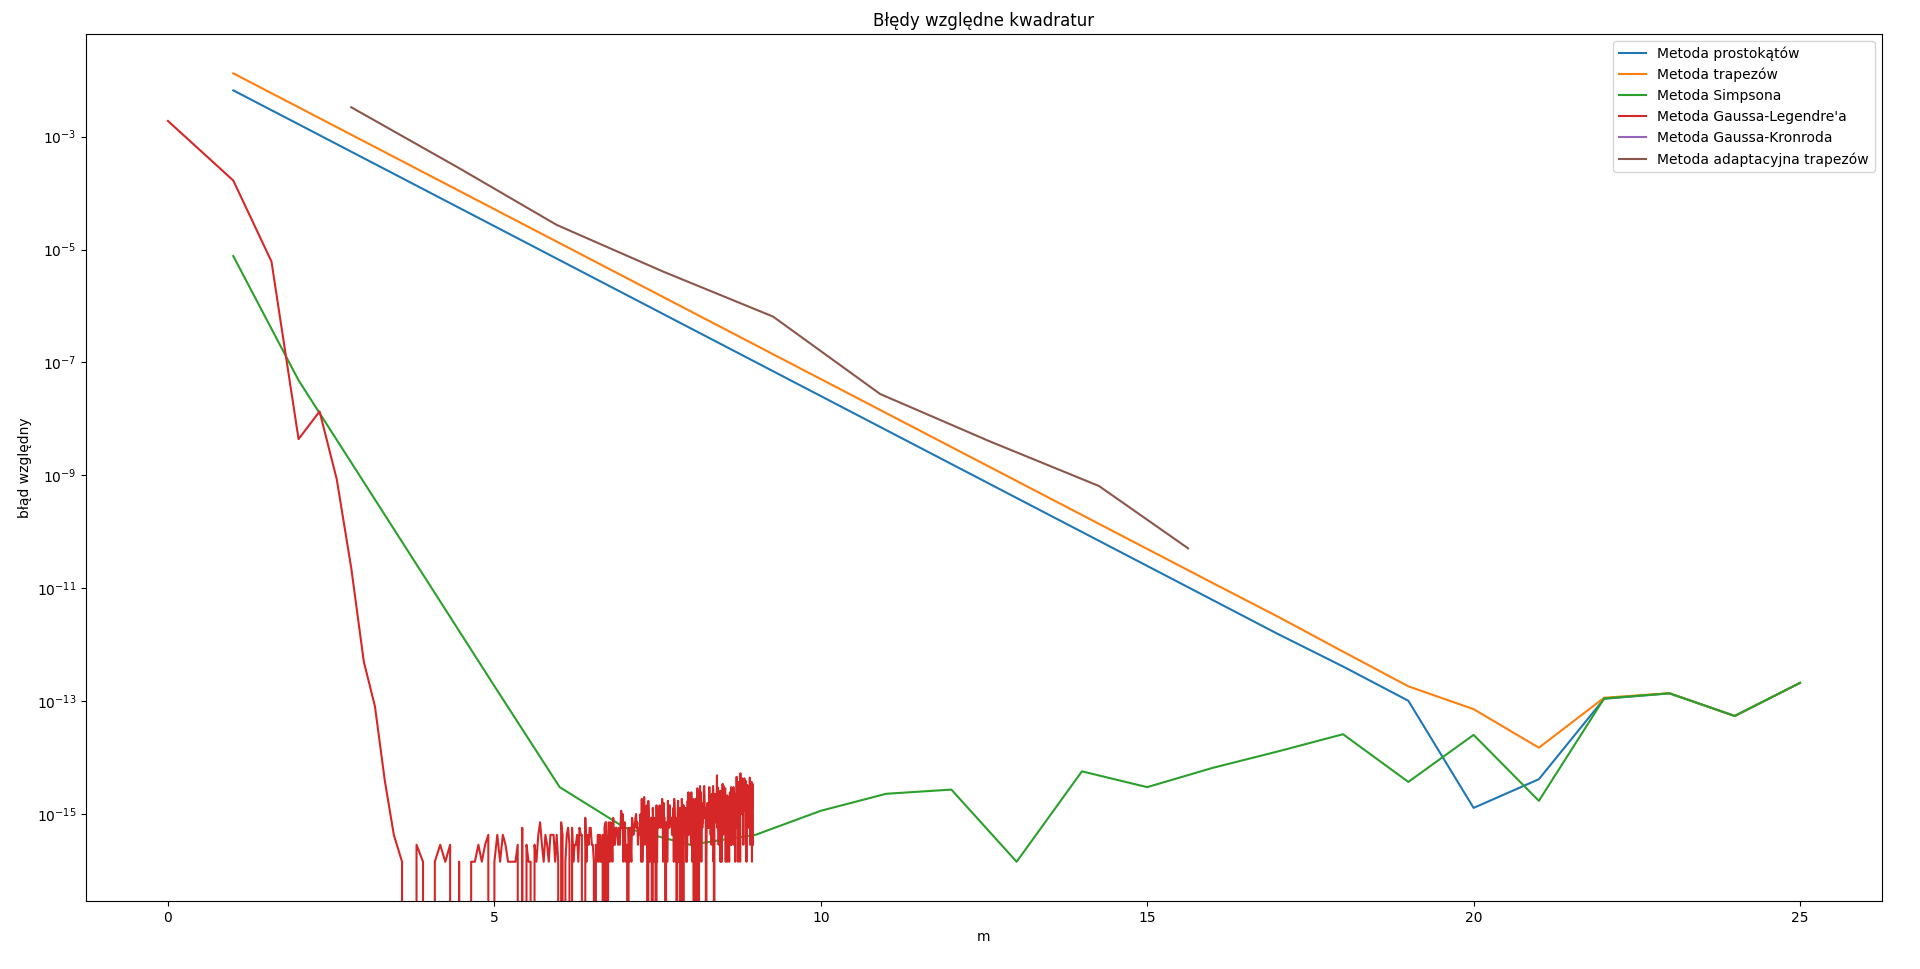
\includegraphics[scale = 0.3]{wykres1.png}
	\end{figure}



	\section*{Zadanie 2}

	\subsection*{Opis problemu}

	Celem zadania było obliczenie wartości następujących całek:

	\begin{equation}
		\int_{0}^{1} \sqrt{x} \log x \,dx
	\end{equation}

	\begin{equation}
		\int_{0}^{1} \left(\frac{1}{(x-0,3)^2+a} + \frac{1}{(x-0,9)^2+b} - 6\right) \,dx
	\end{equation}

	We wzorze przyjęto $a = 0,001$ oraz $b = 0,004$. 

	Wartością dokładną całki ze wzoru (2) są $-\frac{4}{9}$.
	
	Aby wyznaczyć wartość dokładną całki ze wzoru (3), skorzystano z faktu, że:

	\begin{equation}
		\int_{0}^{1} \frac{1}{(x-x_0) + a} \,dx = \frac{1}{\sqrt{a}} \cdot \left(\arctan \frac{1-x_0}{\sqrt{a}} +\arctan \frac{x_0}{\sqrt{a}}\right)
	\end{equation}

	\subsection*{Całkowanie numeryczne}

	W zadaniu należało powtórzyć obliczenia z poprzedniego i aktualnego laboratorium (6 i 7). 

	Zatem skorzystano z metod:
	\begin{itemize}
		\item prostokątów
		\item trapezów
		\item Simpsona
		\item Gaussa-Legendre'a
		\item adaptacyjnych trapezów
		\item Gaussa-Kronroda
	\end{itemize}

	Dla każdej z tych metod obliczono wartość bezwzględną błędu względnego w zależności od liczby ewaluacji. Na podstawie wyników stworzono wykresy zależności tych błędów od $m$:
	
	
	
	
	
	
	
	
	
	
	
	
	
	
\end{document}